\documentclass{article}

\usepackage[pdftex]{graphicx}
\usepackage{smartdiagram}
\usesmartdiagramlibrary{additions}
\usepackage{cleveref}
\usepackage{booktabs} % Allows the use of \toprule, \midrule and \bottomrule in table
\usepackage{xspace,upgreek}
\usepackage{units_definitions}
\usepackage{tikz}
\usepackage{subfig}
% \usepackage[backend=bibtex,style=verbose-trad2]{biblatex}


% *** MATH PACKAGES ***
%
\usepackage{amsmath}

\begin{document}

\title{IDEA drift chamber}
\author{Niloufar Alipour Tehrani}

\maketitle

\section{Introduction}
The FCC-ee high-luminosity circular electron-positron collider, with center-of-mass energies $\sqrt{s}$ from $91.2\,\gev$ to
$365\,\gev$, allows for high-precision measurements of the properties of the Z, the W, the top quark and the Higgs boson. As a predecessor of a new $100\,\tev$ proton-proton collider, the FCC-ee collider is foreseen to be placed in a 100~km tunnel. The IDEA detector, one of the two detector concepts under development for FCC-ee, has demanding requirements to match the experimental conditions. Its main components consist of: an ultra-light silicon-based vertex detector, an ultra-light drift chamber for track reconstruction and particle identification, a double-readout calorimeter, a 2~T solenoid magnetic field and an instrumented return yoke. The drift chamber is being investigated using \textsc{Geant4}-based simulations. Its performance and the effect of beam-induced backgrounds are presented here-below.


\section{Drift chamber}
The parameters of the drift chamber for the IDEA detector is summarized in \cref{driftChamberParams}. A gas, composed of $90~\%$ of Helium and $10~\%$ of isobutane ($\text{C}_{4}\text{H}_{10}$), is foreseen to be used. Thanks to the average stereo angle of 0.1~radians, a longitudinal resolution of 1~mm can be achieved.

\begin{table}[!t]
	\renewcommand{\arraystretch}{1.3}
	\caption{Parameters of the drift chamber for the IDEA detector}
	\label{driftChamberParams}
	\centering
	% Some packages, such as MDW tools, offer better commands for making tables
	% than the plain LaTeX2e tabular which is used here.
	\begin{tabular}{l l}
		\toprule
		Length & 4500~mm \\
        Inner radius & 345~mm \\
        Outer radius & 2000~mm\\
        Number of sensitive wires & 56448 \\
        Single cell resolution (transverse plane) & 0.1~mm \\
		\bottomrule
	\end{tabular}
\end{table}

\section{Simulation with the FCC Software}

The FCC Software (FCCSW)~\cite{FCCSW} is a common software for all FCC experiments. It is based on the Gaudi software framework~\cite{Gaudi} for parallel data processing, \textsc{Geant4} simulation toolkit~\cite{Geant4} and the DD4hep detector description toolkit for high energy physics~\cite{DD4hep}. The FCCSW simulation pipeline is summarized in \cref{simu_chain} and described here-below.

\begin{figure}[!t]
\centering
	\smartdiagramset{back arrow disabled=true}
	\scalebox{1}{
	  	\smartdiagram[flow diagram:horizontal]
	  	{%
	    	{Geometry\\DDhep}, Segmentation, {Geant4 \\simulation}, Digitization%
	  	}
  	}
\caption{The FCCSW simulation chain.}
\label{simu_chain}
\end{figure}


\subsection{Geometry description with DD4hep}
First, the geometry of the detector is described using the DD4hep simulation framework. The implementation of the detectors in the interaction region for the IDEA detector is shown in \cref{fig_sim}. The interaction region consists of a beam pipe, a shielding solenoid, a luminosity calorimeter, a vertex detector and a drift chamber. The geometry of the drift chamber is defined as layers of gas. In order to increase the simulation speed, the individual wires are not physically placed in the simulation software and the segmentation takes them into account.

\begin{figure}[!t]
\centering
    \begin{tikzpicture}
      \node[anchor=south west,inner sep=0] (image) at
      (0,0){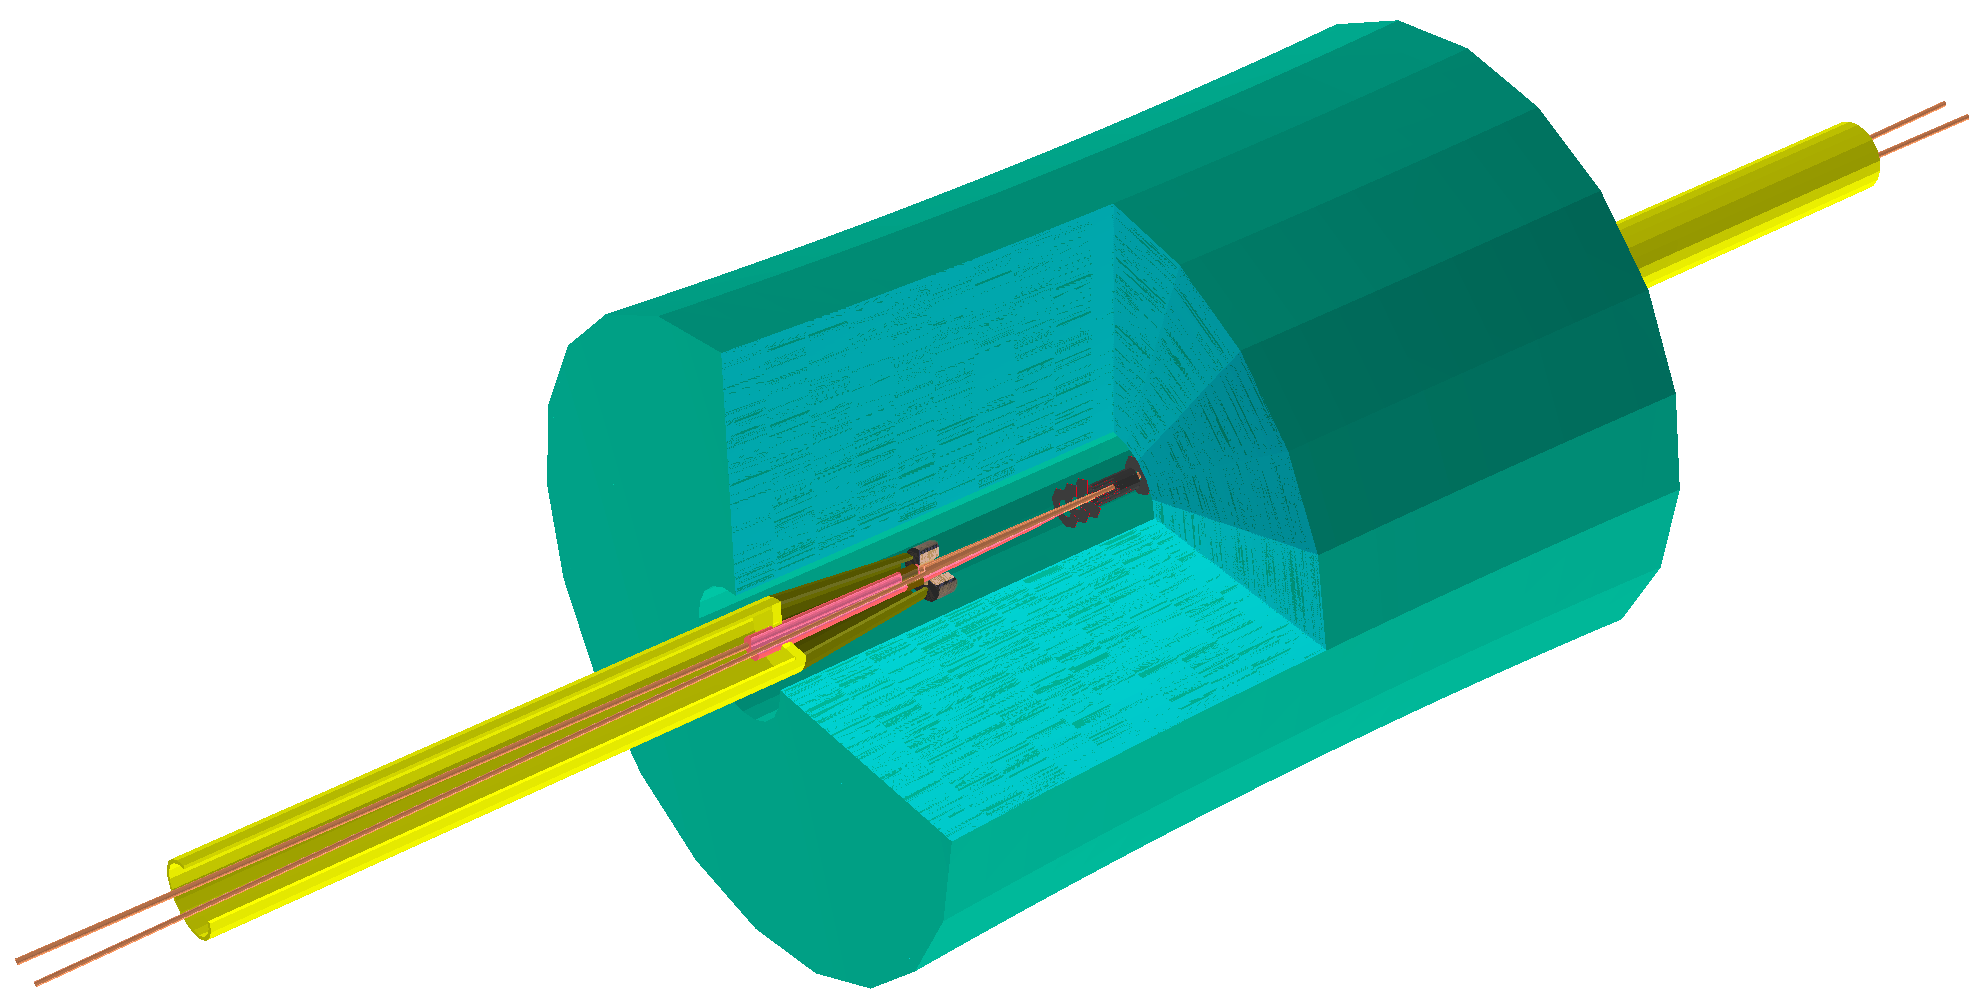
\includegraphics[width=0.8\textwidth]{figures/FCCeeIDEA_IR}};
      \begin{scope}[x={(image.south east)},y={(image.north west)}]

%		\draw[help lines,xstep=.1,ystep=.1] (0, 0) grid (1,1);
%        \foreach \x in {0,1,...,9} { \node [anchor=north] at (\x/10,0) {0.\x}; }
%        \foreach \y in {0,1,...,9} { \node [anchor=east] at (0,\y/10)
%         {0.\y}; }
%
        \draw[->, thick](0.2, 0.7) -- (0.4, 0.7);
		\node[left] at (0.2, 0.7) {Drift chamber};

		\draw[->, thick](-0.1, 0.25) -- (0., 0.25);
		\node[left] at (-0.1, 0.25) {Beam pipe};

		\draw[->, thick](0.1, 0.4) -- (0.2, 0.4);
		\node[left] at (0.1, 0.4) {Solenoid shielding};

		\draw[->, thick](0.6, 0.05) -- (0.48, 0.4);
		\node[below] at (0.6, 0.05) {Luminosity calorimeter};

		\draw[->, thick](0.8, 0.2) -- (0.58, 0.5);
		\node[below] at (0.8, 0.2) {Vertex detector};

	\end{scope}
    \end{tikzpicture}
\caption{The detectors at the interaction region for the FCC-ee IDEA concept.}
\label{fig_sim}
\end{figure}

\subsection{Segmentation}

The segmentation of the sensitive gas detector contains the information on the positions of the wires in the detector. The segmentation for the first layer of the drift chamber is shown in \cref{fig_segmentation_first_case}. The total number of wires as a function of the polar angle $\theta$ is illustrated in \cref{fig_segmentation_second_case}.

\begin{figure}[!t]
\centering
\subfloat[]{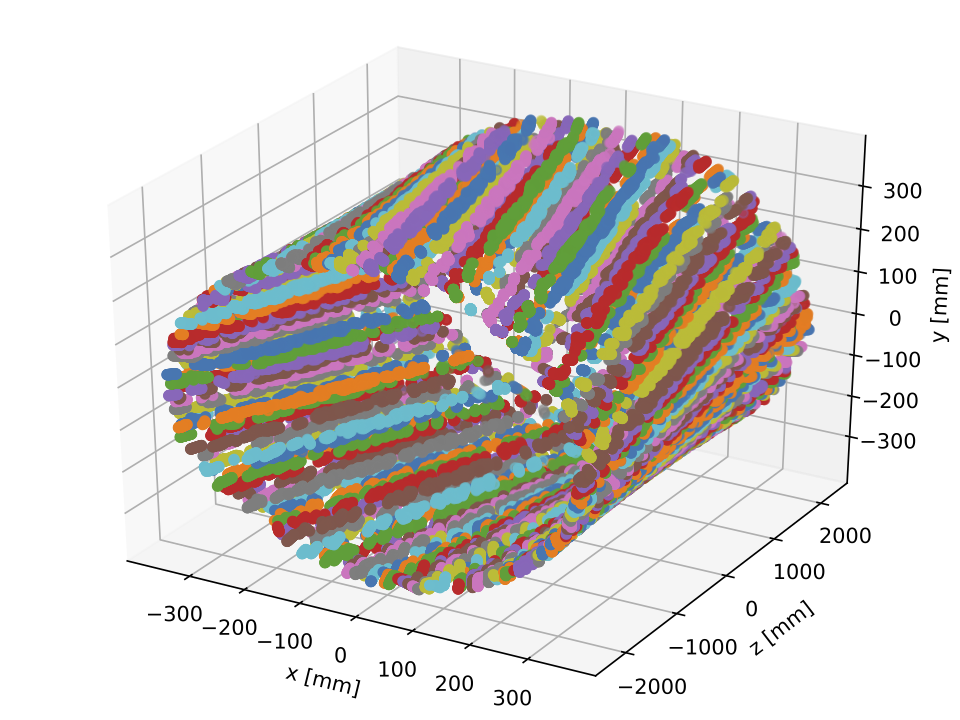
\includegraphics[width=2in]{figures/allHits}%
\label{fig_segmentation_first_case}}
\hfil
\subfloat[]{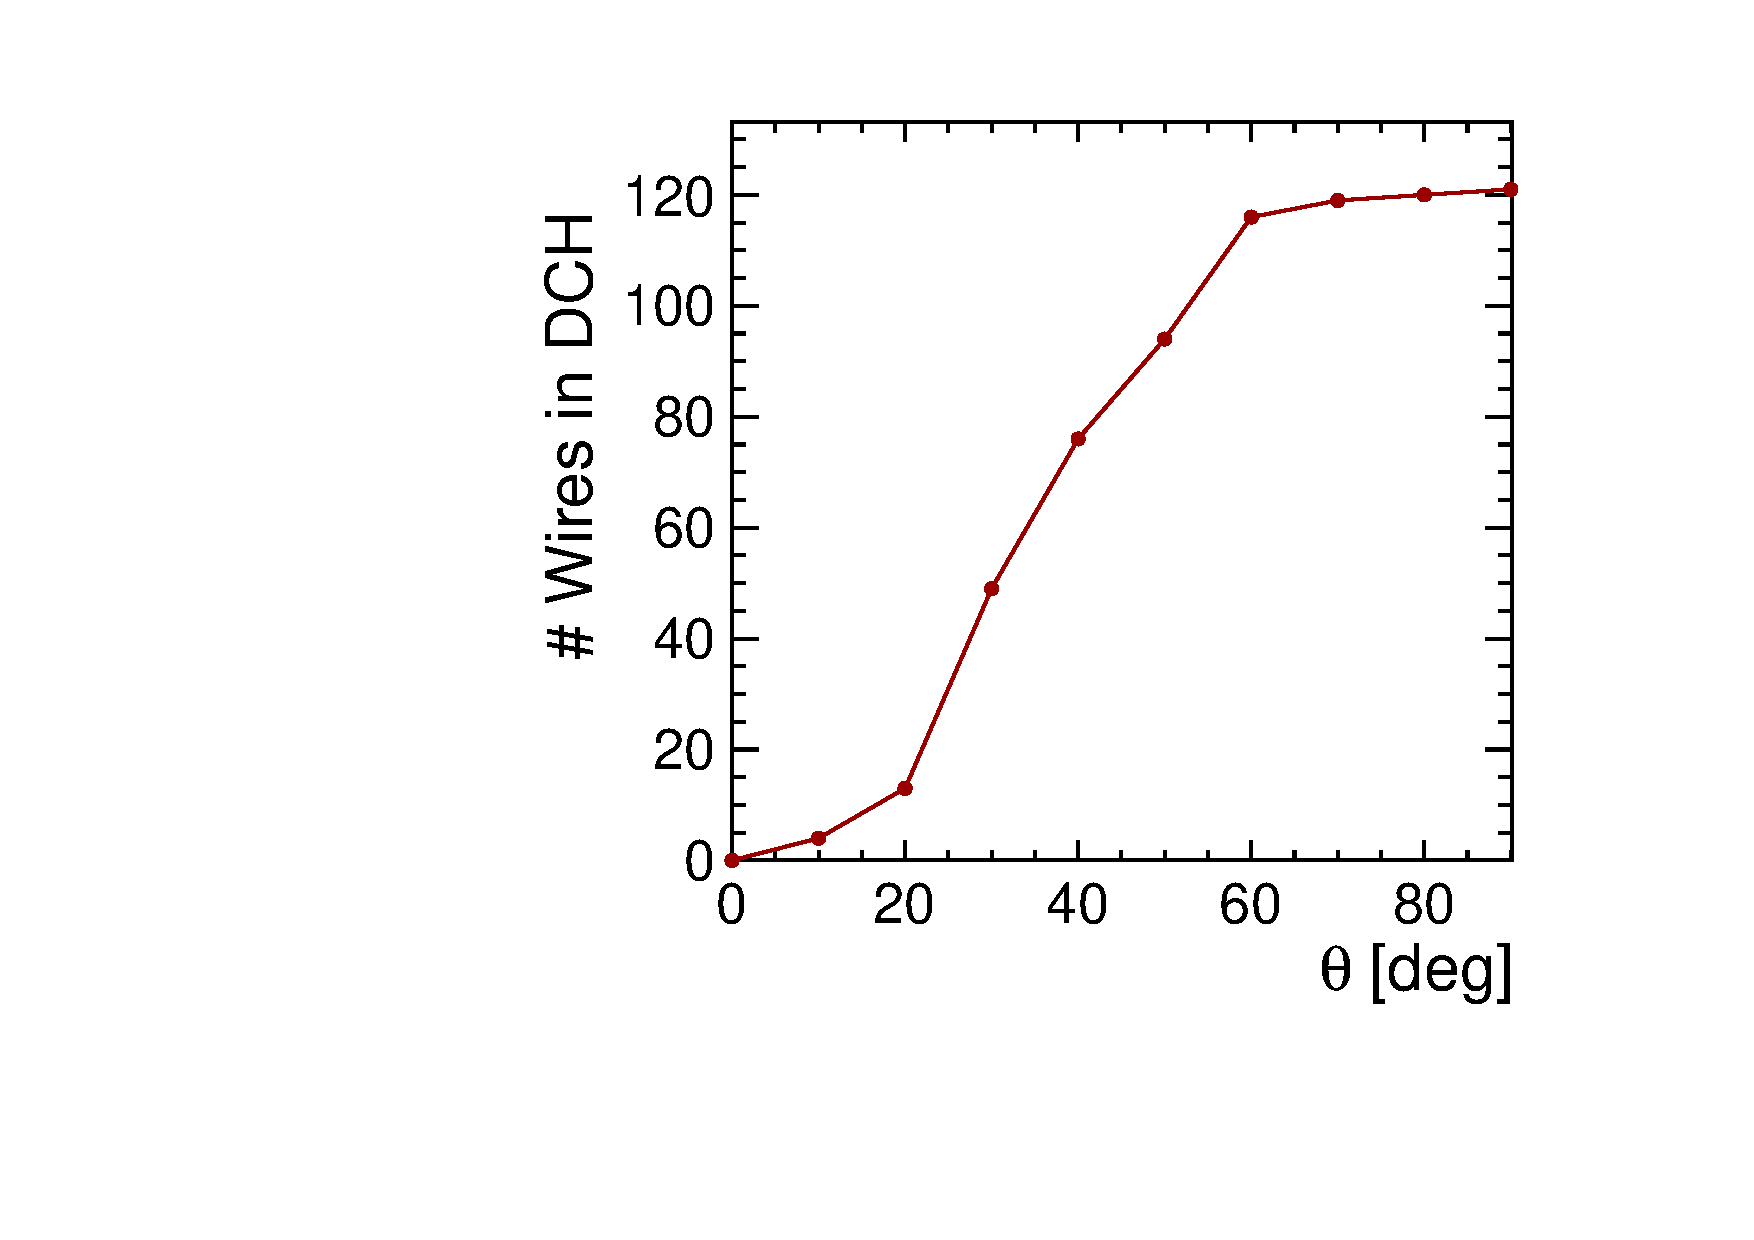
\includegraphics[width=2.5in]{figures/theta_nbHits_DCH}%
\label{fig_segmentation_second_case}}
\caption{(a) shows the segmentation of the first layer of the drift chamber. (b) shows the total number of wires as a function of the polar angle $\theta$ (calculated using infinite momentum tracks from the origin).}
\label{fig_segmentation}
\end{figure}


\subsection{\textsc{Geant4} simulation and digitization}
\textsc{Geant4} simulates the passage of particles through matter. For the drift chamber simulation, a step size of 2~mm is chosen in order to step trough the gas volume and calculate the energy deposited. The ionization charge is then drifted to the nearest wire. This allows for calculating the drift time and therefore the signal in the wires. Once the contribution from each \textsc{Geant4} step is calculated, the digitization step regroups the energy deposited with a drift time smaller than the maximum drift time in the cell.

\section{Impact of beam-induced backgrounds}
One of the main sources of background at the FCC-ee experiments is generated from the strong electromagnetic force from the electron and positron bunches in the field of the opposite beam. This leads to the production of Beamstrahlung photons. The interactions of Beamstrahlung photons generate incoherent lepton pairs at low polar angles and mostly contained in the forward direction as shown in~\cref{fig_pairbcg}. The \textsc{GUINEA-PIG}~\cite{Schulte:382453} event generator has been used to generate the incoherent $e^+e^-$ background particles~\cite{Voutsinas:2017eca} and their impact on the drift chamber is studied below for $\sqrt{s}$ of $92.5\,\gev$ and $365\,\gev$.


\begin{figure}[!t]
\centering
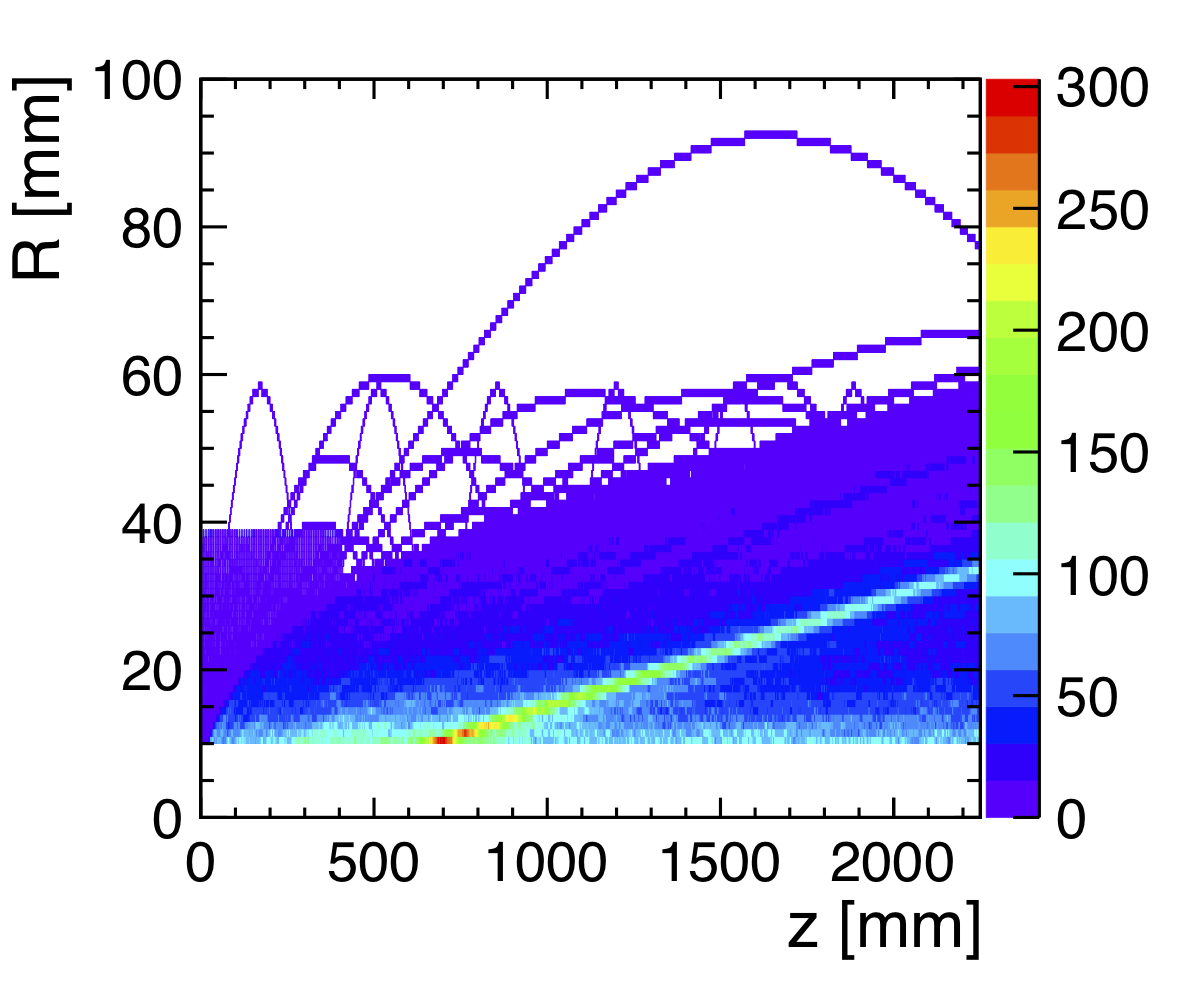
\includegraphics[width=3.5in]{figures/pairs_R_Z.png}
\caption{The trajectory of the $e^+e^-$ pairs in a 2~T magnetic field for a $\sqrt{s}$ of $365\,\gev$.}
\label{fig_pairbcg}
\end{figure}

In fact, the produced incoherent pairs have a low polar angle and only few of them reach the drift chamber. Most of the hits observed are due to the scattering of the $e^+e^-$ pairs by interacting with the elements in the interaction region.

% \begin{figure}[!t]
% \centering
% 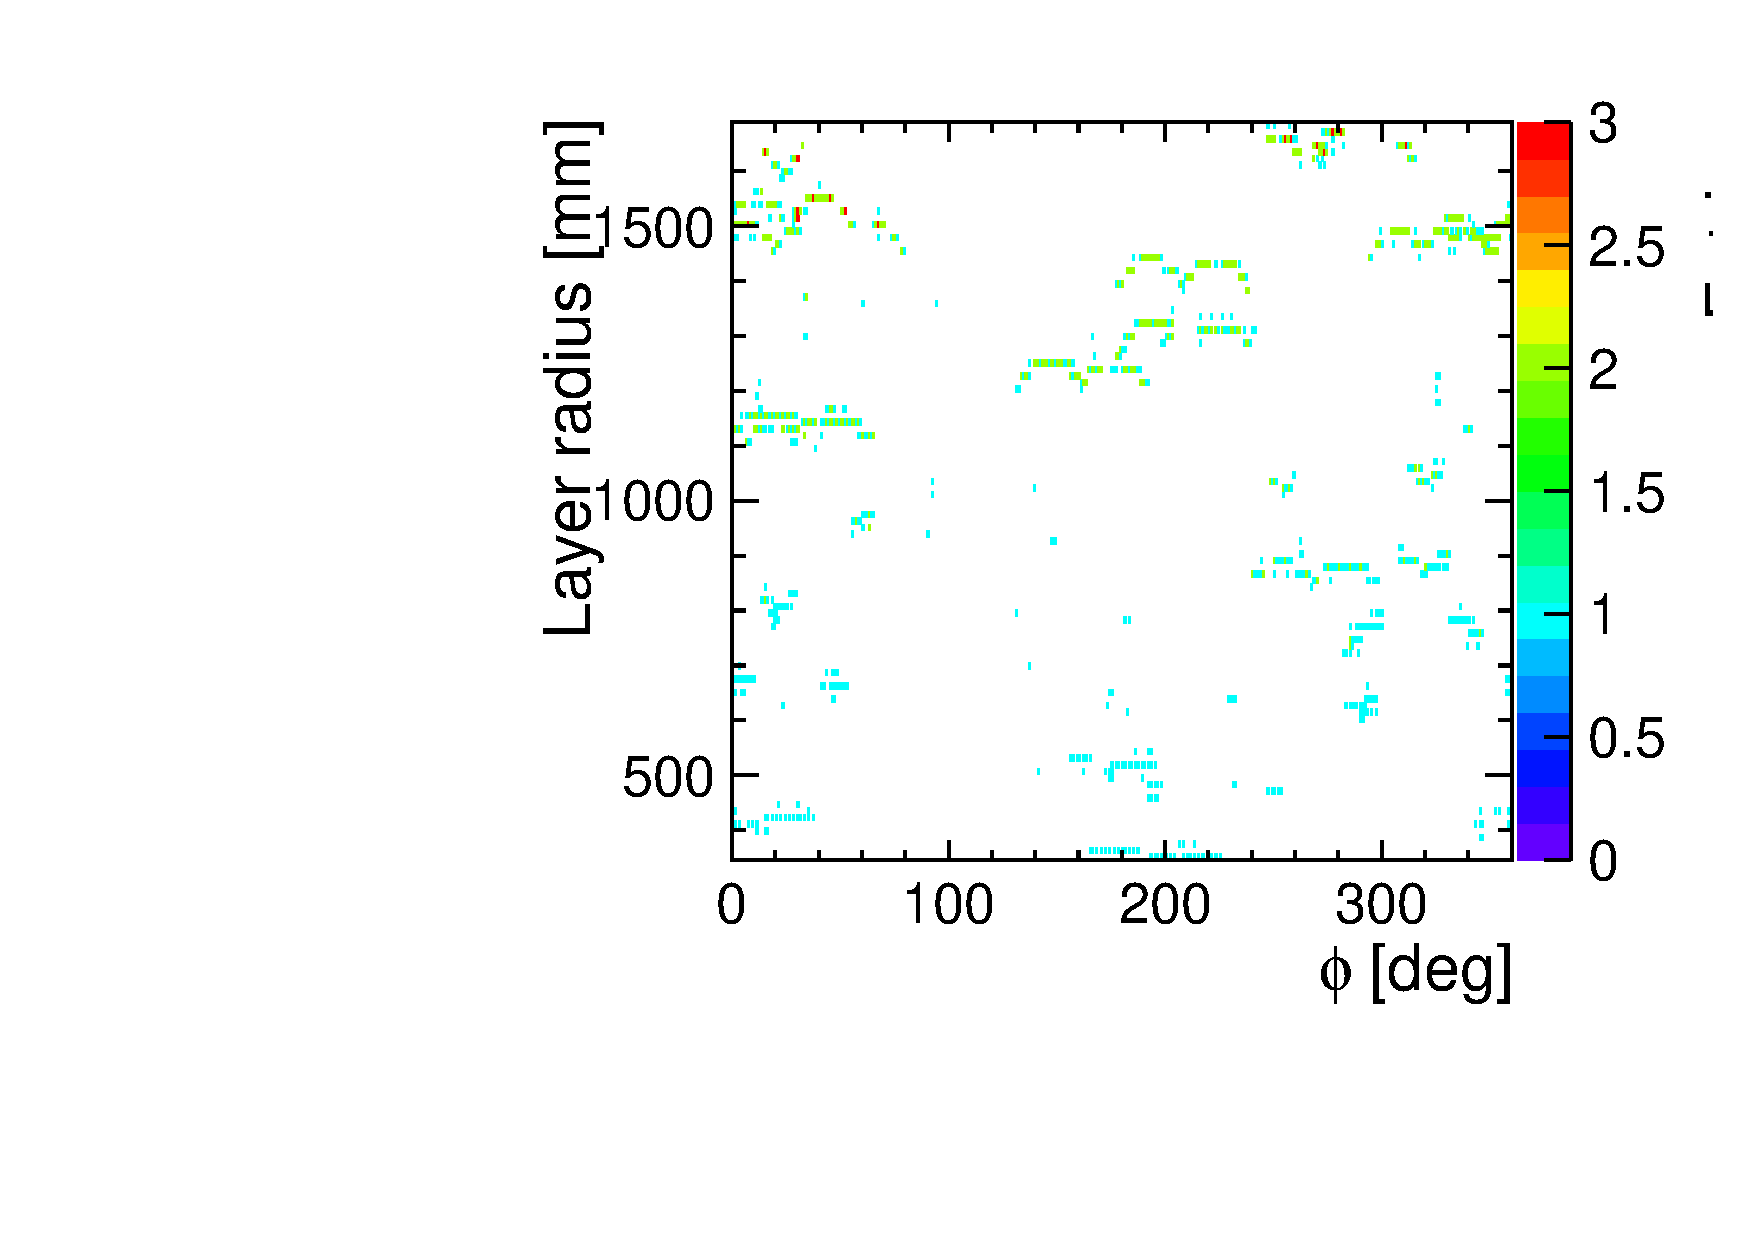
\includegraphics[width=2.5in]{figures/layerR_vs_phi}
% \caption{The detectors at the interaction region for the FCC-ee IDEA concept.}
% \label{fig_simhits}
% \end{figure}

The occupancy of the drift chamber as a function of its radius is shown in~\cref{fig_simhitspercent}. The overall occupancy due to this background remains low and does not pose problems for the reconstruction of the tracks using the drift chamber.

\begin{figure}[!t]
\subfloat[]{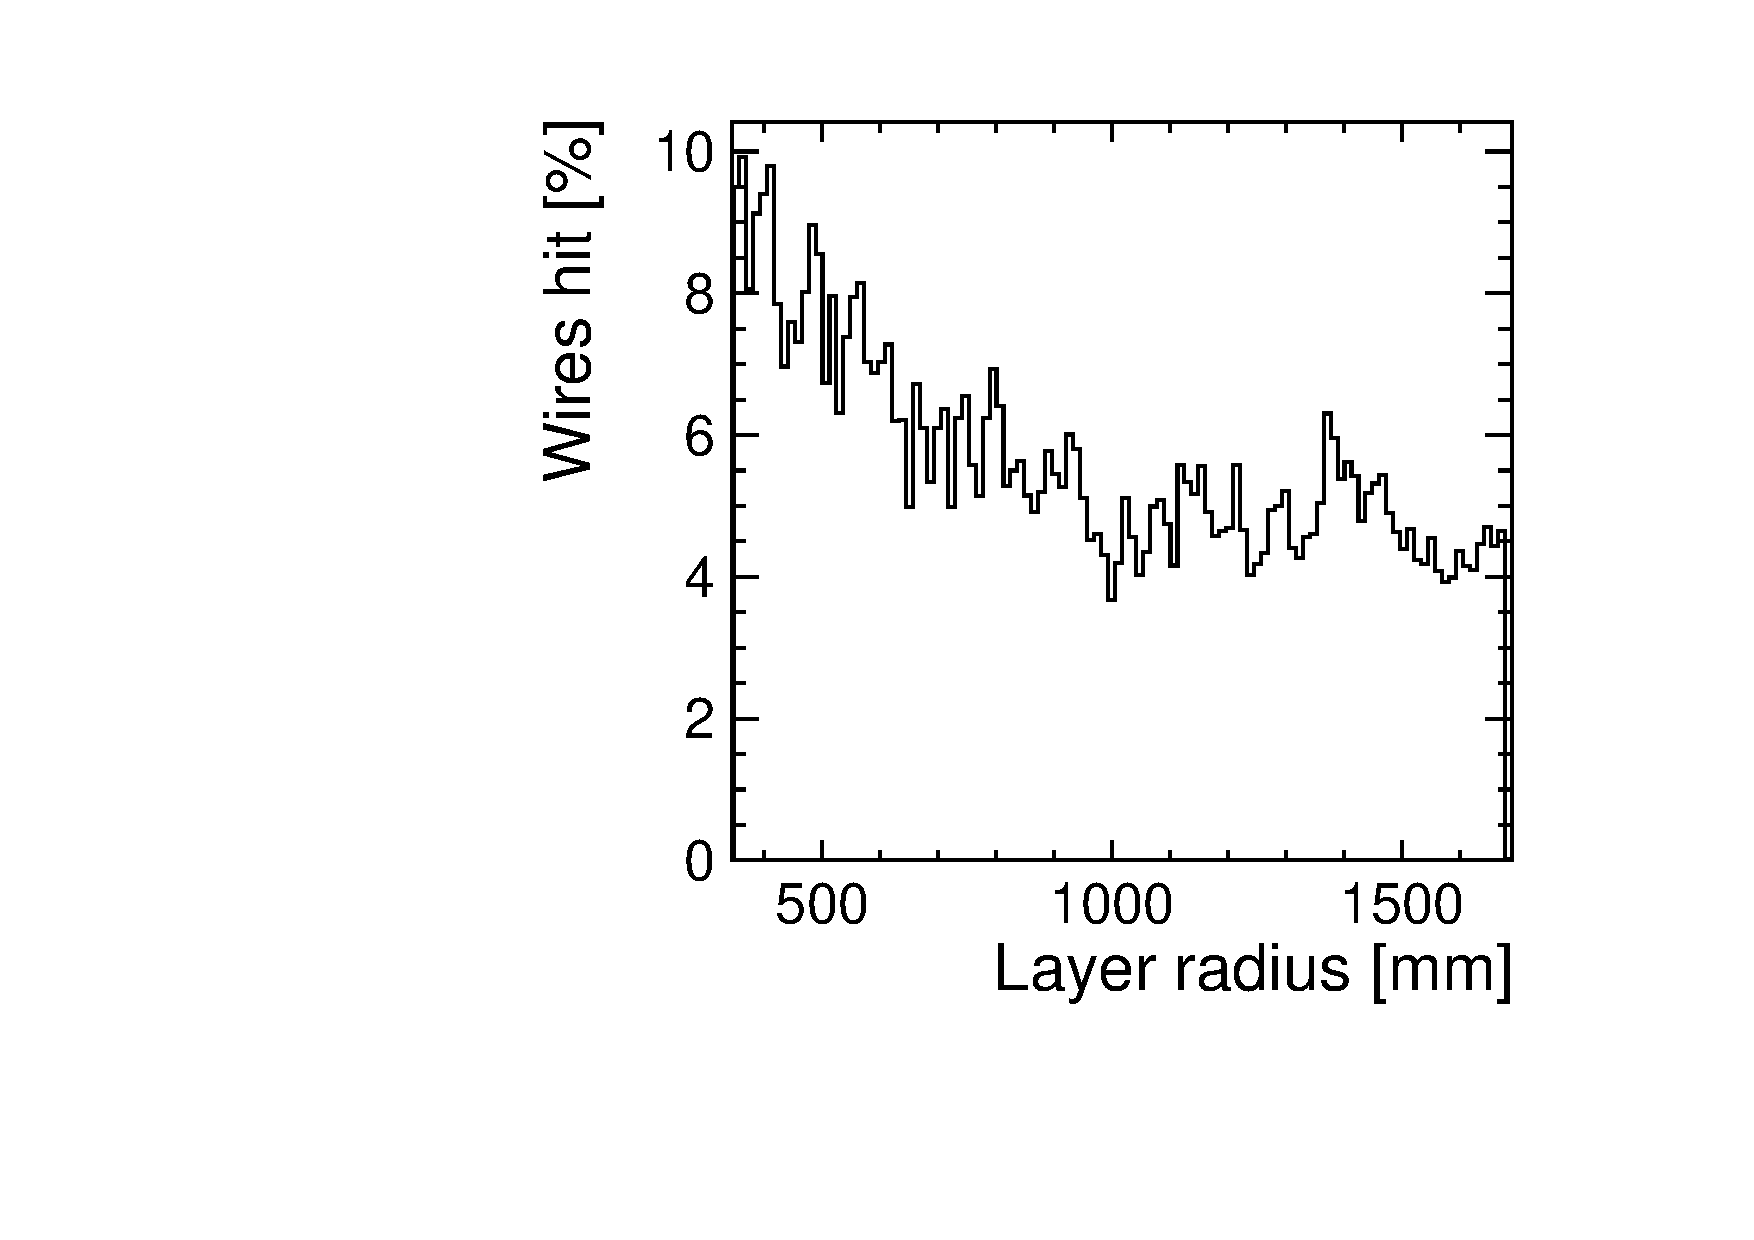
\includegraphics[width=2.5in]{figures/occupancy_Z.pdf}%
% \caption{E\textsubscript{cm}=91.2~GeV}
\label{fig_simhitspercent_Z}}
\hfil
\subfloat[]{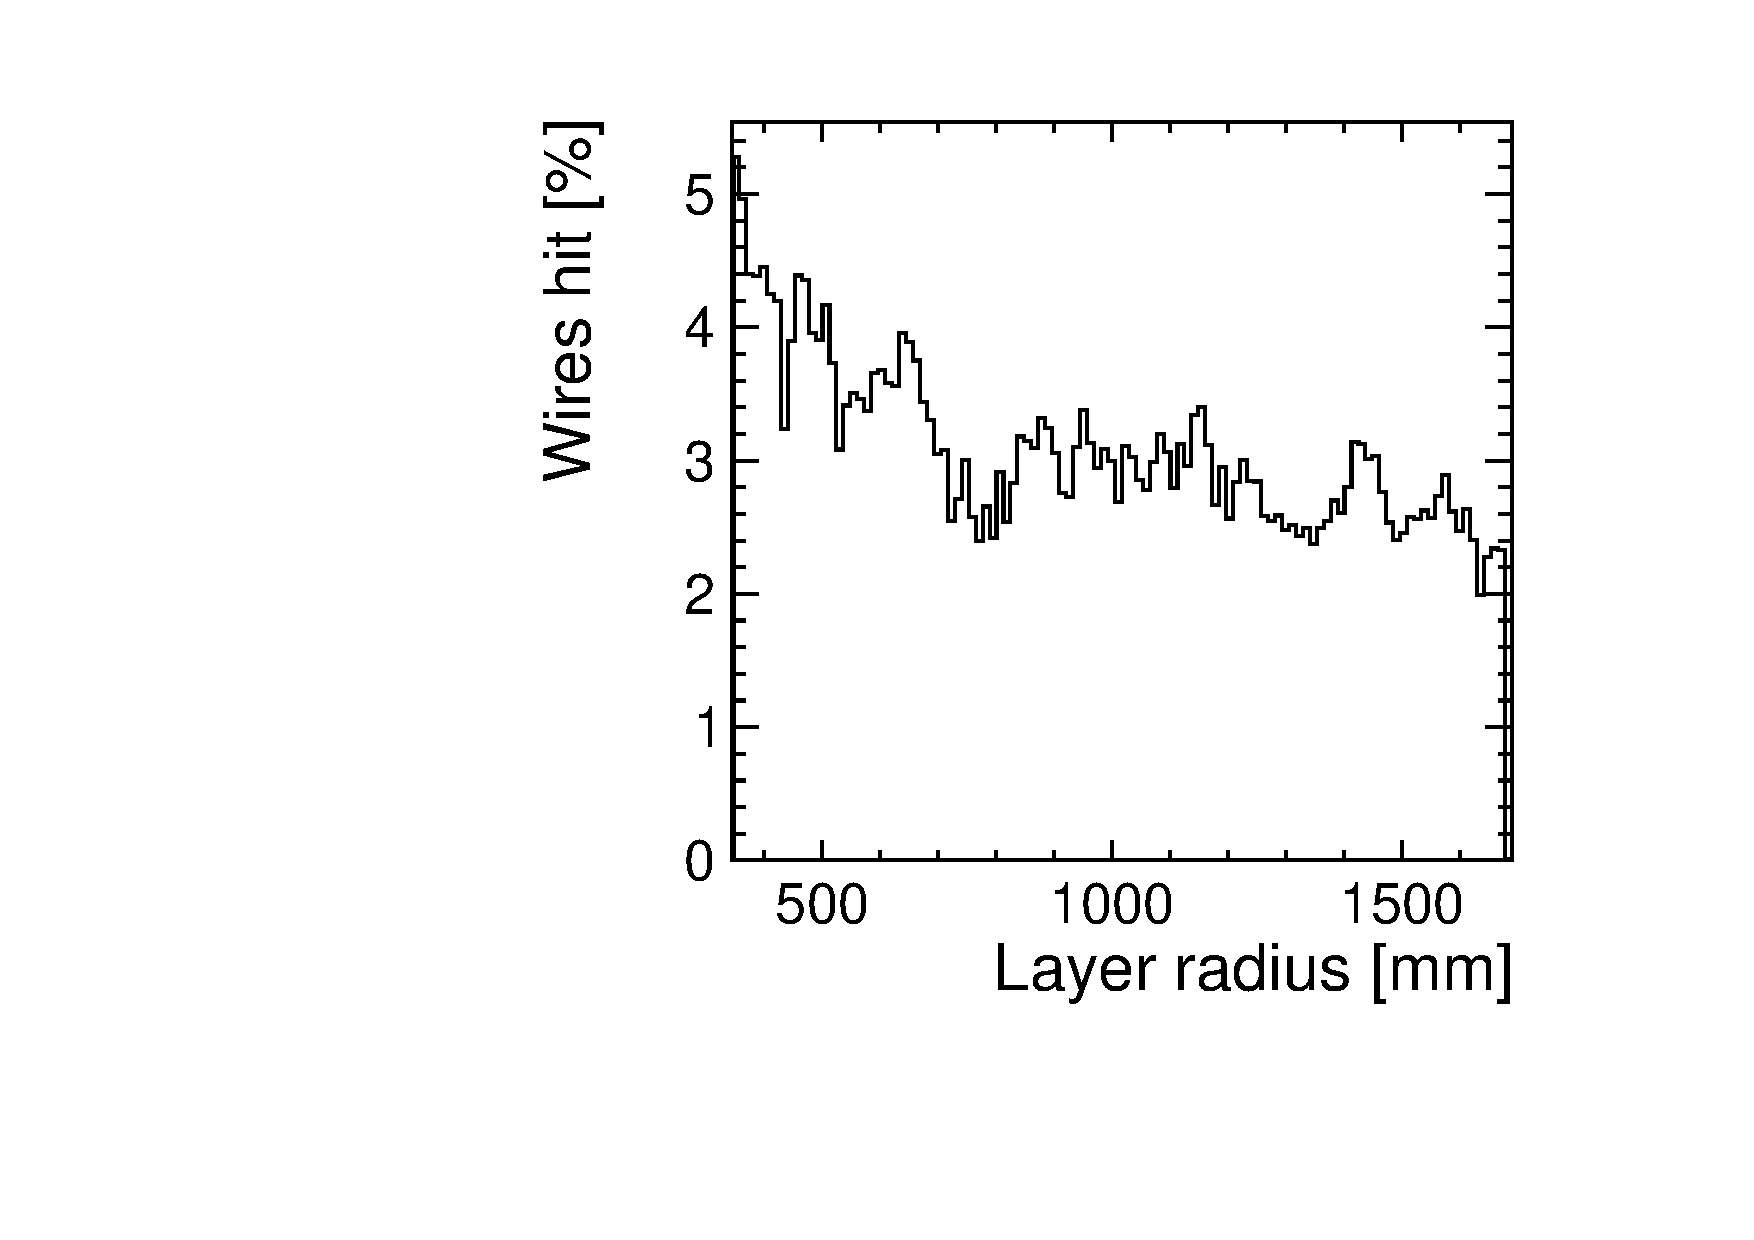
\includegraphics[width=2.5in]{figures/occupancy_top.pdf}%
\label{fig_simhitspercent_top}}
% \centering
% 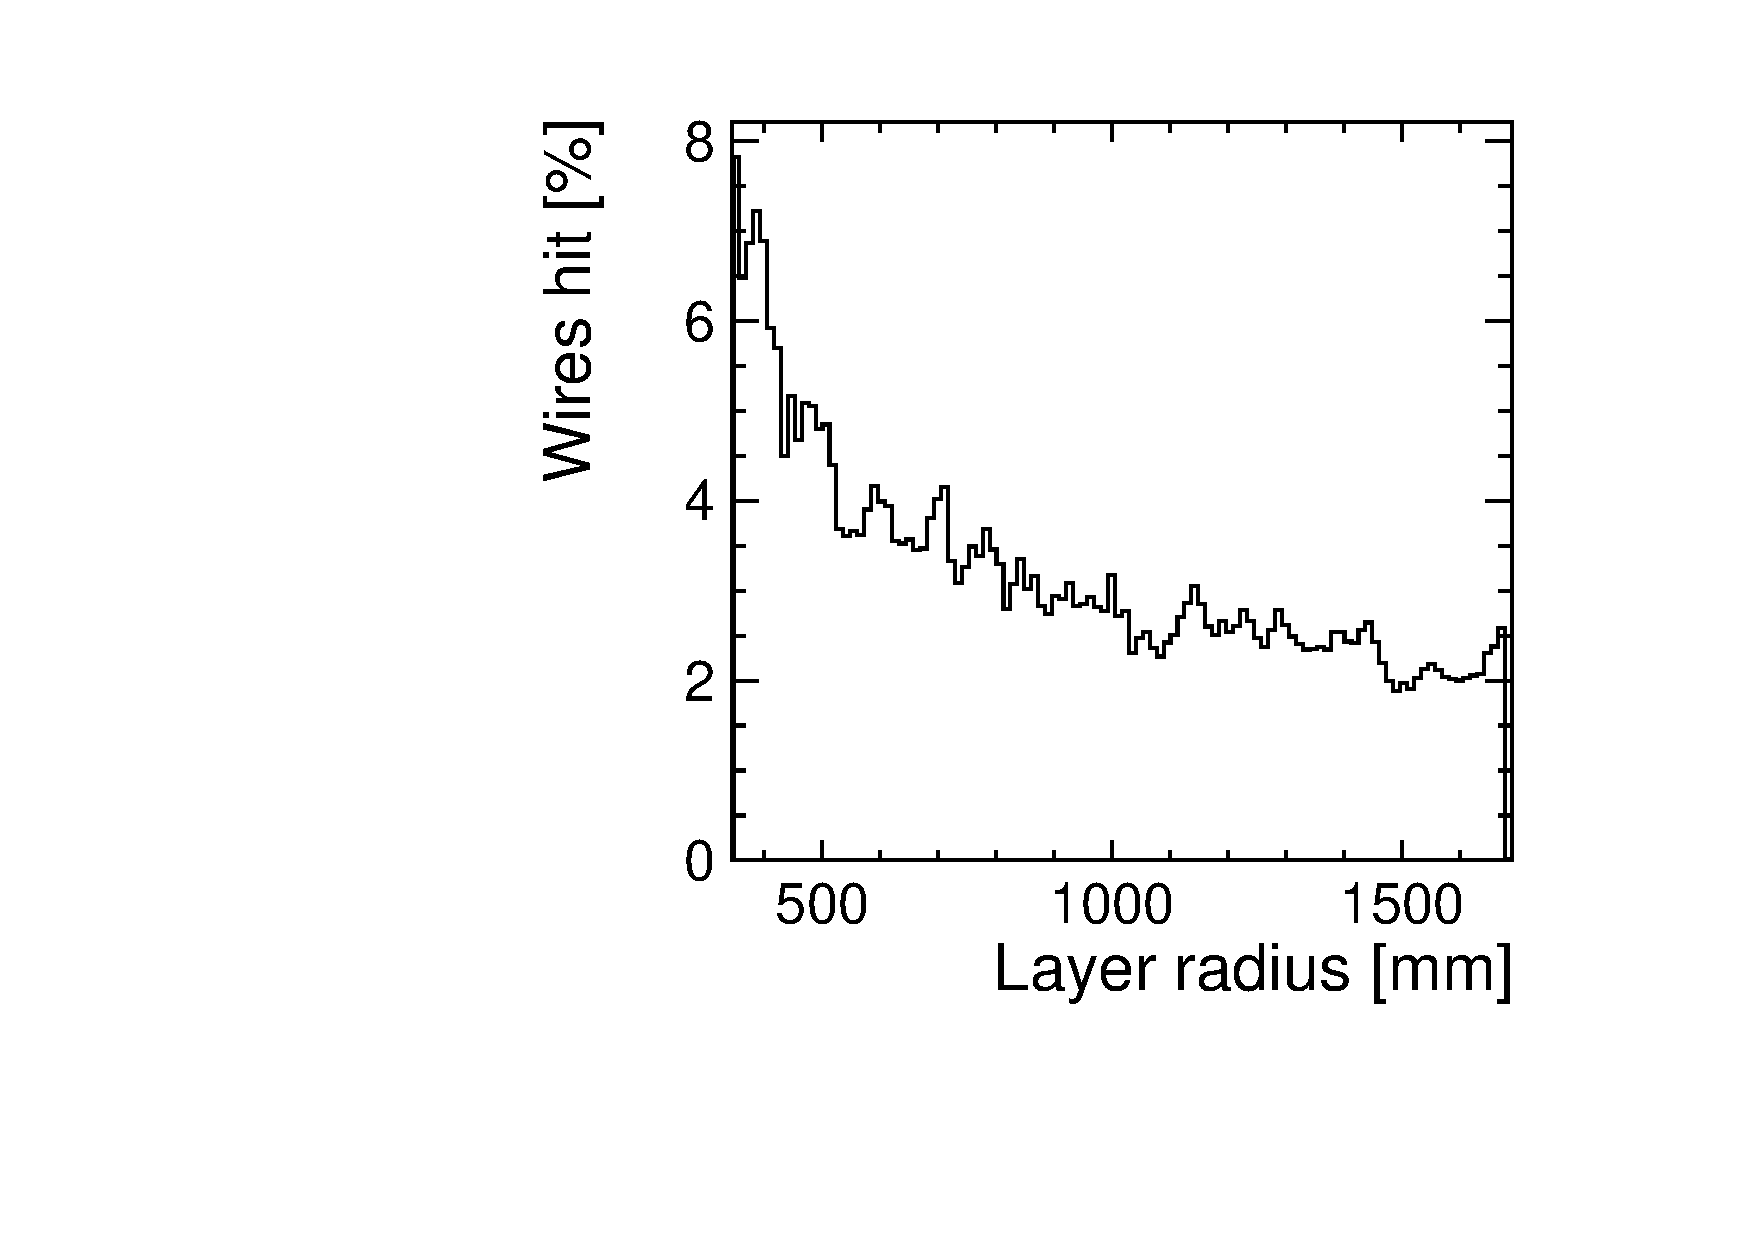
\includegraphics[width=2.5in]{figures/layerR_vs_wires_percent}
\caption{The percentage of wires hit due to $e^+e^-$ background as a function of the layer radius for collisions at (a) $\sqrt{s}$=$92.5\,\gev$ and (b) $\sqrt{s}$=$365\,\gev$.}
\label{fig_simhitspercent}
\end{figure}

\section{Conclusion}
The drift chamber for the IDEA detector concept has been investigated in full simulations using the FCCSW. The full simulation chain has been implemented and validated using this common software and the impact of one of the most important beam-induced backgrounds due to the incoherent $e^+e^-$ pairs has been investigated in simulations. The overall impact remains low and remains promising for the track reconstruction with this detector.

\bibliography{ref.bib}
\bibliographystyle{ieeetr}

\section{Additional checks on the number of wires hit}

\cref{numwires} shows the number of wires hit for 100~GeV single muons at $\theta=90^{\circ}$ uniformly distributed over $\phi$. The distribution contains some tail but the peak corresponds to 112 wires as expected.

\begin{figure}[!t]
\subfloat[]{\includegraphics[width=2.5in]{figures/checkplots/single_muon_90deg.pdf}%
\label{muon90deg}}
\hfil
\subfloat[]{\includegraphics[width=2.5in]{figures/checkplots/single_muon_90deg_zoom.pdf}%
\label{muon90_zoom}}
\caption{Number of wires hit in DCH for 100~GeV muons at $\theta=90^{\circ}$, averaged over $\phi$.}
\label{numwires}
\end{figure}

The number of wires as a function of the polar angle $\theta$ is given in \cref{wires_vs_theta}.

\begin{figure}[!t]
\centering
\subfloat[]{\includegraphics[width=2.5in]{figures/checkplots/nb_layers_DCH_noCut.pdf}%
\label{wires_vs_theta_noCut}}
\hfil
\subfloat[]{\includegraphics[width=2.5in]{figures/checkplots/nb_layers_DCH_ECut100eV.pdf}%
\label{wires_vs_theta_100eVCut}}
\hfil
\subfloat[]{\includegraphics[width=2.5in]{figures/checkplots/nb_layers_DCH_ECut500eV.pdf}%
\label{wires_vs_theta_500eVCut}}
\caption{Number of wires as a function of $\theta$ for (a) no cut on E\textsubscript{dep}, (b) E\textsubscript{dep} $>$ 100~eV and (c) E\textsubscript{dep} $>$ 500~eV.}
\label{wires_vs_theta}
\end{figure}

\section{The distance of closest approach (DCA)}
For 100~GeV single muons, the DCA is being investigated as shown in \cref{DCA_noCut}. The cell sizes, as they are implemented now, vary between $12\times12\,\cmsquared$ and $14\times12\,\cmsquared$. Therefore, the hits in the corners of the cell correspond to a DCA of $\sqrt{12^2+14^2}/2=9.22$~cm.

\begin{figure}[h]
\centering
\subfloat[]{\includegraphics[width=2in]{figures/checkplots/DCA_all.pdf}%
\label{dca_1hit}}
\hfil
\subfloat[]{\includegraphics[width=2in]{figures/checkplots/Edep_tot.pdf}%
\label{Edep_1hit}}
\caption{DCA for 100~GeV muons with a uniform distribution in $\theta$ and $\phi$.}
\label{DCA_noCut}
\end{figure}

The hits having the highest DCAs, have a very low energy deposit and are created due to only one step of \textsc{Geant4}. Their energy deposition is shown in \cref{1hit_DCA_Edep}.

\begin{figure}[h]
\centering
\subfloat[]{\includegraphics[width=2in]{figures/checkplots/DCA_singleHit.pdf}%
\label{dca_1hit}}
\hfil
\subfloat[]{\includegraphics[width=2in]{figures/checkplots/Edep_1hit.pdf}%
\label{Edep_1hit}}
\caption{DCA and E\textsubscript{dep} of hits created due to only one step of \textsc{Geant4}.}
\label{1hit_DCA_Edep}
\end{figure}

By applying a cut of 100~eV, the DCA and the E\textsubscript{dep} within the gas is shown in \cref{DCA_Edep_100eVcut}. This cut reduces the amount of the hits due to signle-Geant4 steps. But on the other hand, the signal is lost.

\begin{figure}[h]
\centering
\subfloat[]{\includegraphics[width=2in]{figures/checkplots/DCA_100eVcut.pdf}%
\label{dca_1hit}}
\hfil
\subfloat[]{\includegraphics[width=2in]{figures/checkplots/Edep_100eVcut.pdf}%
\label{Edep_1hit}}
\caption{DCA and E\textsubscript{dep} by applying a cut of 100~eV on the E\textsubscript{dep}.}
\label{DCA_Edep_100eVcut}
\end{figure}


\end{document}
